
%(BEGIN_QUESTION)
% Copyright 2006, Tony R. Kuphaldt, released under the Creative Commons Attribution License (v 1.0)
% This means you may do almost anything with this work of mine, so long as you give me proper credit

Noen trykkinstrumenter leveres med \textit{kjemiske separasjoner} (chemical seals), bestående av membranenheter koblet til instrumentet med tynne kapillarrør fylt med væske, ofte silikonolje:

$$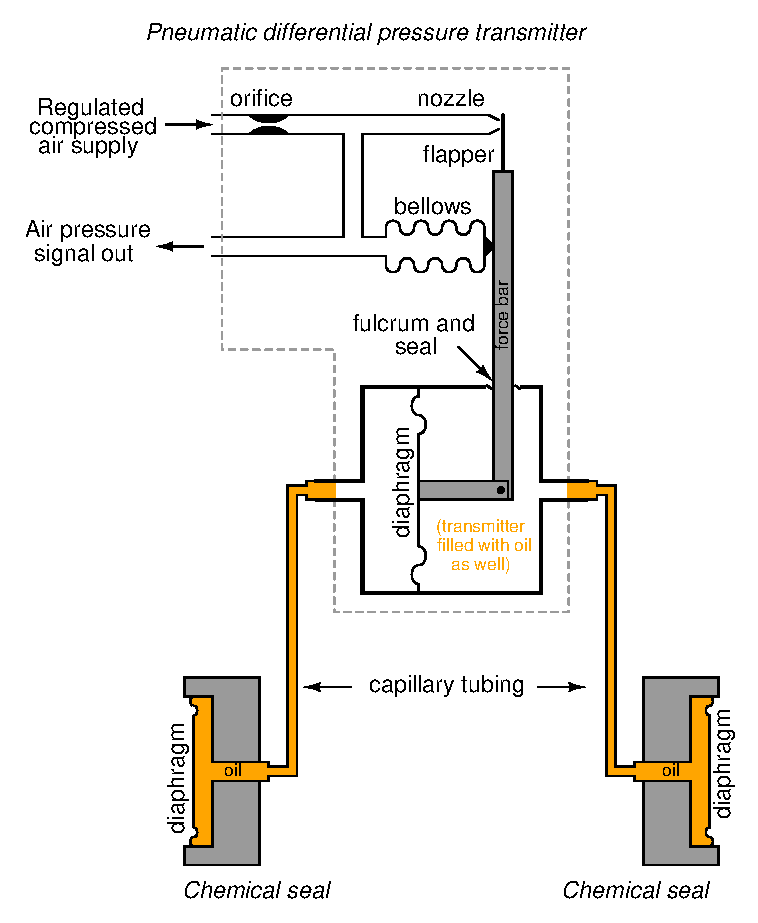
\includegraphics[width=15.5cm]{i00216x01.eps}$$

\filbreak

Disse kan så kobles til prosesstank for trykkmåling, med avstand mellom transmitter og prosess:

$$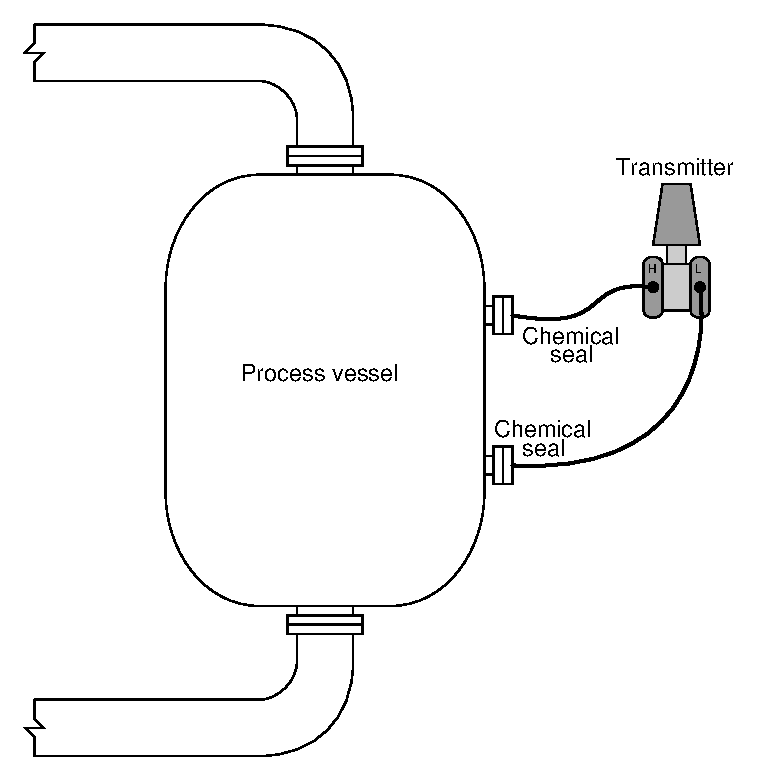
\includegraphics[width=15.5cm]{i00216x02.eps}$$

Hvilke formål har slike separasjoner?  Hvilke fordeler gir de ved trykkmåling?

\underbar{file i00216}
%(END_QUESTION)





%(BEGIN_ANSWER)

Remote chemical seals gjør det mulig for trykktransmittere å måle trykket i svært korrosive prosessmedier.  De eneste delene i kontakt med prosessmediet er selve seal-elementene: hus og membraner.  Kapillarrørene mellom seals og transmitter inneholder kun ren olje, det samme gjør transmitteren.

Et naturlig spørsmål er: hvorfor bruke fjernmembran mot prosessen i stedet for å bygge hele transmitteren av samme materiale?  Svaret er blant annet at transmittere (spesielt bevegelsesbalanserte typer) er begrenset i hvilke materialer selve trykkelementet kan lages av.  Trykkelementet må ha gode elastiske egenskaper, noe som ofte begrenser materialvalg.  Seal-membraner er derimot ``slakke'' og skal i praksis ikke bidra med fjærmotstand, bare overføre trykket.  Derfor er elastiske egenskaper mindre kritiske der, og materialvalget kan optimaliseres for korrosjonsbestandighet.

Selv hvis både seal-membran og sensorelement er metalliske, finnes det gode grunner for chemical seals.  Med vanlig fjernmontert transmitter kreves impulsrør fra prosess til transmitter.  Materialvalg for slike instrumentrør er ofte mer begrenset enn for seal-membraner, og rørene kan være svakeste ledd mot korrosjon.  Remote seals med oljefylte kapillarrer løser dette ved å holde prosessmediet ute av rør og transmitter.

En annen grunn er hygieniske prosesser (mat/farma), der lommer med stillestående væske ikke er akseptable.  Vanlig DP-kapsel og impulsrør kan skape hulrom for bakterievekst.  Flushmonterte remote seals gir plan prosessflate og overfører trykket via fill-væske uten bakterietilgang.

Tilsvarende brukes remote seals for å redusere plugging.  Vanlige impulsrør kan tettes av sediment eller partikler, mens flushmonterte seals ikke gir samme oppsamlingssteder.

%(END_ANSWER)





%(BEGIN_NOTES)


%INDEX% Measurement, pressure: chemical seals
%INDEX% Measurement, pressure: remote seals

%(END_NOTES)

